\chapter{Evaluation}
\label{eval}

Now that we have discussed the goals and scope of the proof-of-concept implementation of MM-quecat, recall that in~\cref{quecat}, we mentioned query performance as one of the main open points of our approach.
In~\cref{category:section:querylanguage}, we mentioned that a suitable multi-model query language should \textit{"have the capability of being nearly as performant as native queries where possible"}.
To that end, we discussed optimization options in~\cref{algorithms} while discussing the proposed algorithms.
However, in order to properly understand the performance of the proposed approach, and to be able to constructively suggest effective optimizations for the future, it would be useful to experimentally evaluate the performance of MM-quecat.
This chapter is therefore dedicated to such an evaluation.

Specifically, we have four main goals in mind for the experiments in this chapter, which is to:

\begin{enumerate}
    \item Understand the overhead introduced by our approach compared to native database queries in a single-model scenario;
    \item Understand the overhead in the context of merging data in a multi-model, multi-database scenario;
    \item Locate the main performance bottlenecks in MM-quecat; and
    \item Establish a performance baseline for future optimizations.
\end{enumerate}

The motivations for the first goal should be quite clear, as our approach introduces overhead in the form of converting data into a categorical representation and network communication overhead.
Therefore to properly fulfill the first goal of this chapter, we will need to prepare simple, single-model scenarios which we can use to isolate the amount of overhead introduced in this fashion.

As for the second goal, recall that in~\cref{algorithms}, we mentioned the need to merge together data retrieved from different query parts.
While the merging itself is not performed directly by MM-quecat, but rather by MM-evocat~\cite{evocat}, it is still crucial to understand the impact of this step on the whole approach.
To this end, we will naturally need to include a multi-model scenario in our evaluation.

Lastly, a simple observation motivates the third goal - in practice, it is best to avoid premature optimization, and rather use benchmarking to identify specific performance bottlenecks.
Because the problem domain of multi-model querying is very complex, naturally the approaches we designed are as well.
This means that avoiding premature optimization is even more important, as we want to preserve the simplicity and comprehensibility of our approach where possible.
To this end, during the writing of this chapter, two key tools were utilized to aid us in locating performance bottlenecks: Python's cProfile\footnote{\url{https://docs.python.org/3/library/profile.html}} module which allows us to collect performance statistics about Python programs, and SnakeViz\footnote{\url{https://jiffyclub.github.io/snakeviz/}}, which is a tool for the visualization of cProfile's output.

Before we begin with the evaluation itself, it is also worth mentioning that the use cases designed for evaluation purposes also serve as use cases for the verification of the implementation of MM-quecat.
Specifically, the multi-model use case presented in~\cref{eval:section:multimodel} also presents the main use case of MM-quecat (and this thesis in general), which is the unified querying of multi-model data.
By including this use case in the evaluation, we also verify that MM-quecat fulfills its intended primary purpose.

\section{Evaluation Framework}

\begin{figure}[h]
\centering
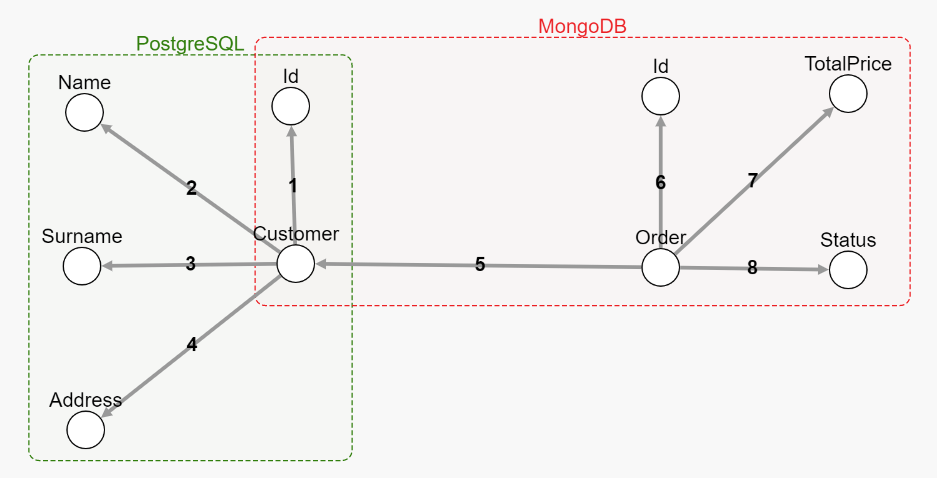
\includegraphics[width=\textwidth]{img/eval-category.png} 
\caption{Schema category used for all evaluations.}
\label{fig:evalcategory}
\end{figure}

For the purposes of the aforementioned evaluations, we propose a model scenario used for both single-model and multi-model evaluations.
The schema category for this scenario is shown in~\cref{fig:evalcategory}.
The corresponding mappings are then shown in~\cref{fig:evalmapping}.
The customers along with their properties are stored in a PostgreSQL table, and the orders are stored in a MongoDB collection.
Using this schema, we are able to easily test the multi-model functionality of MM-quecat while keeping the example simple and understandable.
Note that the \texttt{customer\_id} stored for each order in MongoDB refers to a customer stored in PostgreSQL, allowing the joining of the data.

For each evaluation scenario, the given MMQL query is executed, timed, and its execution time is compared to the execution time of a native database query (or two native queries in the case of the multi-model scenario).
Each scenario was repeated 100 times, and the presented results are the average of all repetitions.

The choice of databases for this example scenario is also not random - MM-evocat~\cite{evocat} supports only PostgreSQL and MongoDB, and therefore MM-quecat does as well.
Therefore the only reasonable option is to use both the supported databases if we want to examine the multi-model behavior.

\begin{figure}[h]
\centering
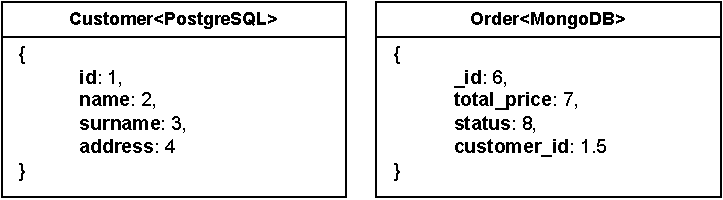
\includegraphics[width=\textwidth]{img/eval-mappings.pdf} 
\caption{Mappings corresponding to the schema category in~\cref{fig:evalcategory}.}
\label{fig:evalmapping}
\end{figure}

Every proper test needs a well-defined set of input data, and it is no different for our case.
The data was generated using the Faker\footnote{\url{https://faker.readthedocs.io/en/master/}} library, using a random seed for reproducibility.
As for the size of the data, a set of 2000 customers and 6000 orders was used, with each customer being assigned 3 orders.

The evaluations were performed on a laptop with an 11th generation Intel i7 CPU, 32 gigabytes of operating memory and an SSD.
Both databases as well as the MM-evocat instance were running locally on the same machine, using Docker\footnote{\url{https://www.docker.com/}} for virtualization.

It is also worth reminding that even though there is a single multi-model schema for all evaluations, we are able to use specific parts of it for the single-model evaluations.

All evaluations described in this chapter are part of the MM-quecat source code\footnote{\url{https://github.com/yawnston/querycat}} as executable Python scripts in the \texttt{src/experiments} folder.

\section{Single-Model Evaluation}

As mentioned in the introduction of this chapter, the purpose of single-model evaluation is to isolate the overhead introduced by our approach compared to native database queries.
In a single-model scenario, we do not need to consider the overhead of merging together data from multiple different databases, and we can focus on only the base overhead.
A separate evaluation was carried out for both currently supported databases - PostgreSQL and MongoDB.

\subsection{PostgreSQL}
\label{eval:subsection:postgresql}

In the PostgreSQL evaluation, let us consider a query which simply selects all customers along with their properties, using the schema shown in~\cref{fig:evalcategory}.
Such a MMQL query is shown in~\cref{fig:evalpostgresqlmmql}.

\begin{figure}[ht]
\begin{code}
SELECT {
    ?customer id ?id ;
        name ?name ;
        surname ?surname ;
        address ?address .
}
WHERE {
    ?customer 1 ?id ;
        2 ?name ;
        3 ?surname ;
        4 ?address .
}
\end{code}
\caption{MMQL query used for PostgreSQL single-model evaluation.}\label{fig:evalpostgresqlmmql}
\end{figure}

We also consider an equivalent PostgreSQL query shown in~\cref{fig:evalpostgresqlnative}, which was used as the benchmarking query.
When compared to the query shown in~\cref{fig:evalpostgresqlgenerated}, which was internally generated by MM-quecat for the given MMQL query, we can see that they are functionally identical.

\begin{figure}[ht]
\begin{code}
SELECT id, name, surname, address
FROM experiments_customers
\end{code}
\caption{PostgreSQL query used for benchmarking performance.}
\label{fig:evalpostgresqlnative}
\end{figure}

\begin{figure}[ht]
\begin{code}
SELECT 
  experiments_customers.id AS experiments_customers_id, 
  experiments_customers.name AS experiments_customers_name, 
  experiments_customers.surname AS experiments_customers_surname, 
  experiments_customers.address AS experiments_customers_address 
FROM 
  experiments_customers
\end{code}
\caption{PostgreSQL query generated by MM-quecat from the query shown in~\cref{fig:evalpostgresqlmmql}.}
\label{fig:evalpostgresqlgenerated}
\end{figure}

The results of this evaluation scenario can be seen in~\cref{table:evalpostgresqlresults}, with the first row showing the raw elapsed query time in milliseconds, and the second row showing slowdown relative to the native query.
We can see that on average, the MMQL query took a little over 1 second to execute, compared to just 4ms for the native query, giving us a slowdown of roughly 288 times.

\begin{table}[h!]
\centering
\begin{tabular}{l@{\hspace{1.5cm}} c c}
& \textbf{Native Query} & \textbf{MM-evocat} \\
\midrule
Elapsed Time & 4ms & 1153ms \\
Slowdown & 1x & 288x \\
\bottomrule
\end{tabular}
\caption{Average query time measurements for the single-model PostgreSQL scenario.}\label{table:evalpostgresqlresults}
\end{table}

This degree of slowdown was within the realm of expectation, because we need to consider the overhead of communication with the MM-evocat instance, as well as the overhead of transforming the data into a categorical representation.
However, what is more interesting is to take a look at where the majority of the slowdown is coming from.
Looking at~\cref{fig:evalpostgresqlprofile}, we can see performance measurement data collected by cProfile and visualized by SnakeViz\footnote{The profiler run was done separately from the performance measurement runs shown in~\cref{table:evalpostgresqlresults} in order to eliminate any possible performance effect of the profiler itself.}.
This data shows a visualization of the total execution time spent in given function calls, starting at the top and decomposing the function calls further as we go down in the image.

\begin{figure}[h]
\centering
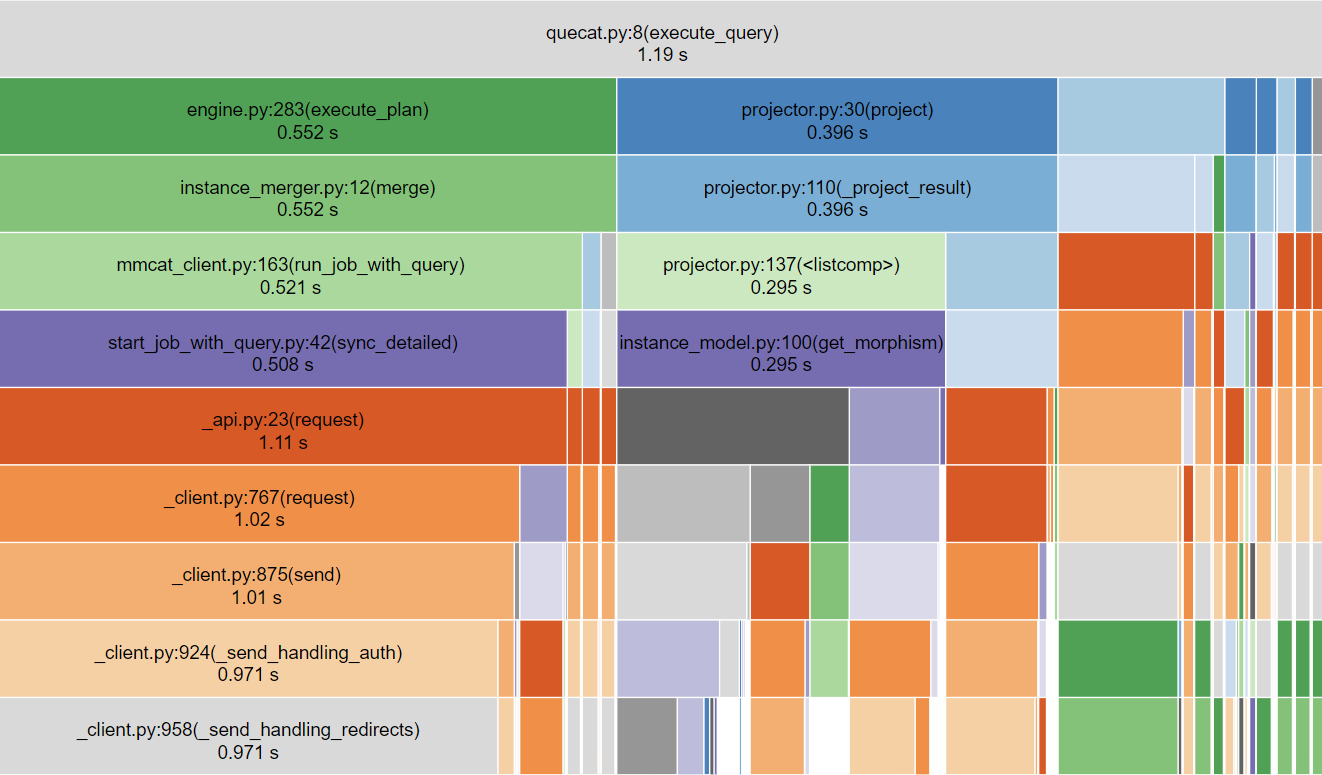
\includegraphics[width=\textwidth]{img/eval-postgre-profile.png} 
\caption{Profiler data for the single-model PostgreSQL scenario.}
\label{fig:evalpostgresqlprofile}
\end{figure}

Some function names are omitted from the image due to the available space, but examining the data contained within reveals the main takeaway of this evaluation scenario: the majority of the time was spent on \textbf{network communication} with MM-evocat.
This network communication necessarily includes the transfer of all retrieved data from MM-evocat to MM-quecat.
In other words, the amount of time spent otherwise manipulating the data was trivial.
This gives us a good baseline idea of the performance of MM-quecat, as we can expect that execution times for arbitrary queries will likely not go too far below 1 second.

The only feasible way of reducing this overhead further would be to revise the architecture of the ecosystem including MM-evocat and MM-quecat, and to merge them together into a single tool.
However, that would be far from trivial, considering the relevant tools were developed independently as part of different theses using different languages. Such an endeavor may not be worth the performance benefits at this point of the tools' lifecycle.
Perhaps if in the future a highly performant variant of both MM-evocat and MM-quecat is desired, a new, unified tool can be built from scratch using the knowledge gained from the design and implementation of both tools.

\subsection{MongoDB}
\label{eval:subsection:mongodb}

Similarly to~\cref{eval:subsection:postgresql}, this evaluation scenario evaluates MM-quecat in the context of a single data model within a single database.
The evaluated MMQL query for this scenario is shown in~\cref{fig:evalmongodbmmql}, the benchmark MongoDB query is shown in~\cref{fig:evalmongodbnative}.
The query generated by MM-quecat is identical to the query shown in~\cref{fig:evalmongodbnative}, therefore it is not shown in a separate figure.

\begin{figure}[ht]
\begin{code}
SELECT {
    ?order id ?orderId ;
        totalPrice ?totalPrice ;
        status ?status ;
        customerId ?customerId .
}
WHERE {
    ?order 6 ?orderId ;
        7 ?totalPrice ;
        8 ?status ;
        5/1 ?customerId .
}
\end{code}
\caption{MMQL query used for MongoDB single-model evaluation.}\label{fig:evalmongodbmmql}
\end{figure}

\begin{figure}[ht]
\begin{code}
db.experiments_orders.aggregate([
    {
        "$project": {
            "_id": 1,
            "total_price": 1,
            "status": 1,
            "customer_id": 1
        }
    }
])
\end{code}
\caption{MongoDB query used for benchmarking performance, identical to the query generated by MM-quecat.}
\label{fig:evalmongodbnative}
\end{figure}

The results of this evaluation scenario can be seen in~\cref{table:evalmongodbresults}.
We can see that the average execution time for the native MongoDB query was 16ms, while the average for MM-evocat was 5458ms.
This gives us an approximate slowdown of 341x.

\begin{table}[h!]
\centering
\begin{tabular}{l@{\hspace{1.5cm}} c c}
& \textbf{Native Query} & \textbf{MM-evocat} \\
\midrule
Elapsed Time & 16ms & 5458ms \\
Slowdown & 1x & 341x \\
\bottomrule
\end{tabular}
\caption{Average query time measurements for the single-model MongoDB scenario.}\label{table:evalmongodbresults}
\end{table}

The measurements show an increase in the overhead incurred by MM-evocat, and the reason for this becomes apparent when examining~\cref{fig:evalmongodbprofile}.
As we can see, network communication between MM-evocat and MM-quecat now only takes up approximately 30\% of the total query execution time.
The remaining 70\% is taken up by work being done in the \texttt{QueryProjector} class, specifically by the method \texttt{\_contract\_morphisms}.

Recall that in~\cref{algo:subsection:projection}, we discussed the projection algorithm, including the need for so-called morphism \textit{contractions}.
A morphism contraction is an operation on the instance category, where we may need to contract multiple instance morphisms into a single one because of the required projection in the query.
This is an operation which for $m$ morphisms with data size $n$ effectively requires $m-1$ joins between instance morphism domain rows, where each instance morphism may contain up to $n$ domain rows.
These joins are implemented using a linear number of operations and a hash table in MM-quecat, however there may be room for optimization here.
Perhaps a more efficient contraction algorithm could be designed, eliminating the need for hashing by clever usage of memory layout for the data being joined.
Similarly, the representation of the instance category is not optimized for performance, therefore there may be some room for improvement here as well.
In any case, the instance morphism contractions form a major performance bottleneck in MM-quecat, along with the serialization and deserialization of the instance category also having room for optimization.

\begin{figure}[h]
\centering
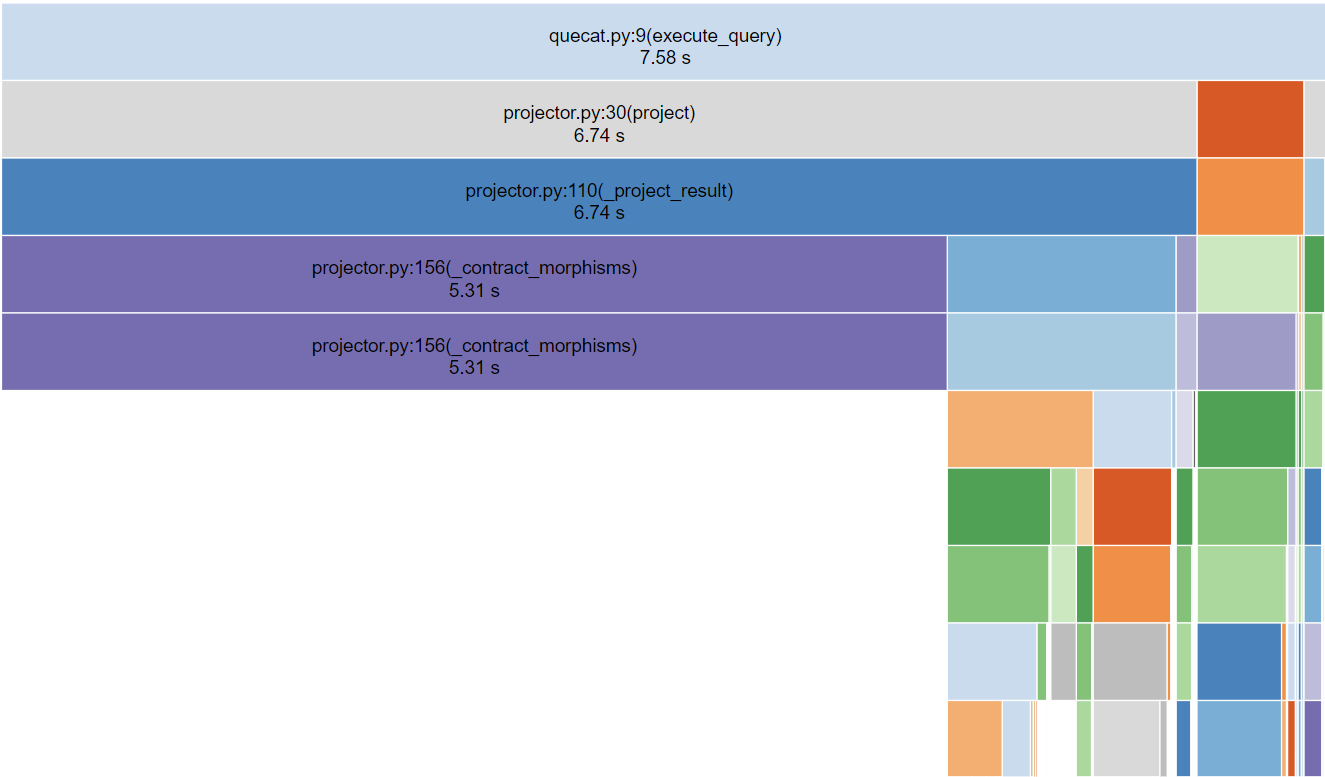
\includegraphics[width=\textwidth]{img/eval-mongodb-profile.png} 
\caption{Profiler data for the single-model MongoDB scenario.}
\label{fig:evalmongodbprofile}
\end{figure}

The reader may be wondering why we did not see this effect of the contractions in~\cref{eval:subsection:postgresql}.
The reason for this can be seen in the structure of the MMQL query itself - the query in this scenario contains the triple \texttt{?order 5/1 ?customerId}, but this compound morphism is contracted into a single base morphism in the \texttt{SELECT} clause.
For that reason, the contractions are needed in this instance, whereas in~\cref{eval:subsection:postgresql}, no such operation was needed due to the structure of the query.

\section{Multi-Model Evaluation}
\label{eval:section:multimodel}

In the previous section, we examined the characteristics of MM-quecat in the context of querying a single database at a time.
However, one of the main benefits of MM-quecat and MMQL is the ability to uniformly query data from multiple databases at a time.
Also, recall that one of the goals for this chapter was to understand the overhead in the context of merging data in a multi-model, which we have not yet done.
This is why this last evaluation scenario is focused on MM-quecat in a multi-model context.

\begin{figure}[ht]
\begin{code}
SELECT {
    ?order id ?orderId ;
        totalPrice ?totalPrice ;
        status ?status ;
        customerName ?customerName ;
        customerSurname ?customerSurname ;
        address ?customerAddress .
}
WHERE {
    ?order 6 ?orderId ;
        7 ?totalPrice ;
        8 ?status ;
        5 ?customer .

    ?customer 2 ?customerName ;
        3 ?customerSurname ;
        4 ?customerAddress .
}
\end{code}
\caption{MMQL query used for multi-model evaluation.}\label{fig:evalmultimodelmmql}
\end{figure}

Recall~\cref{fig:evalcategory}, which shows the schema category used in these evaluations.
In this scenario, we will finally be using the entire schema category.
The MMQL query in~\cref{fig:evalmultimodelmmql} selects data for each order from MongoDB, while also selecting customer data from PostgreSQL and joining the data based on the customer ID stored with the orders.

As this is a multi-model scenario, we will be running queries in both PostgreSQL and MongoDB, and their combined elapsed time form the performance baseline.
These baseline queries are the same as in the previous section (i.e. \cref{fig:evalpostgresqlnative} and \cref{fig:evalmongodbnative}), we will just be using both of them at the same time.
We will also not be showing the queries generated by MMQL in this instance, as they are virtually identical to the generated queries in the previous scenarios.

\begin{table}[h!]
\centering
\begin{tabular}{l@{\hspace{1.5cm}} c c}
& \textbf{Native Queries} & \textbf{MM-evocat} \\
\midrule
Elapsed Time & 46ms & 19209ms \\
Slowdown & 1x & 417x \\
\bottomrule
\end{tabular}
\caption{Average query time measurements for the multi-model scenario.}\label{table:evalmultimodelresults}
\end{table}

The results for this final scenario are shown in~\cref{table:evalmultimodelresults}.
We can see that the native queries combined took approximately 46 milliseconds on average, whereas MM-evocat finished its work in around 19 seconds.

\begin{figure}[h]
\centering
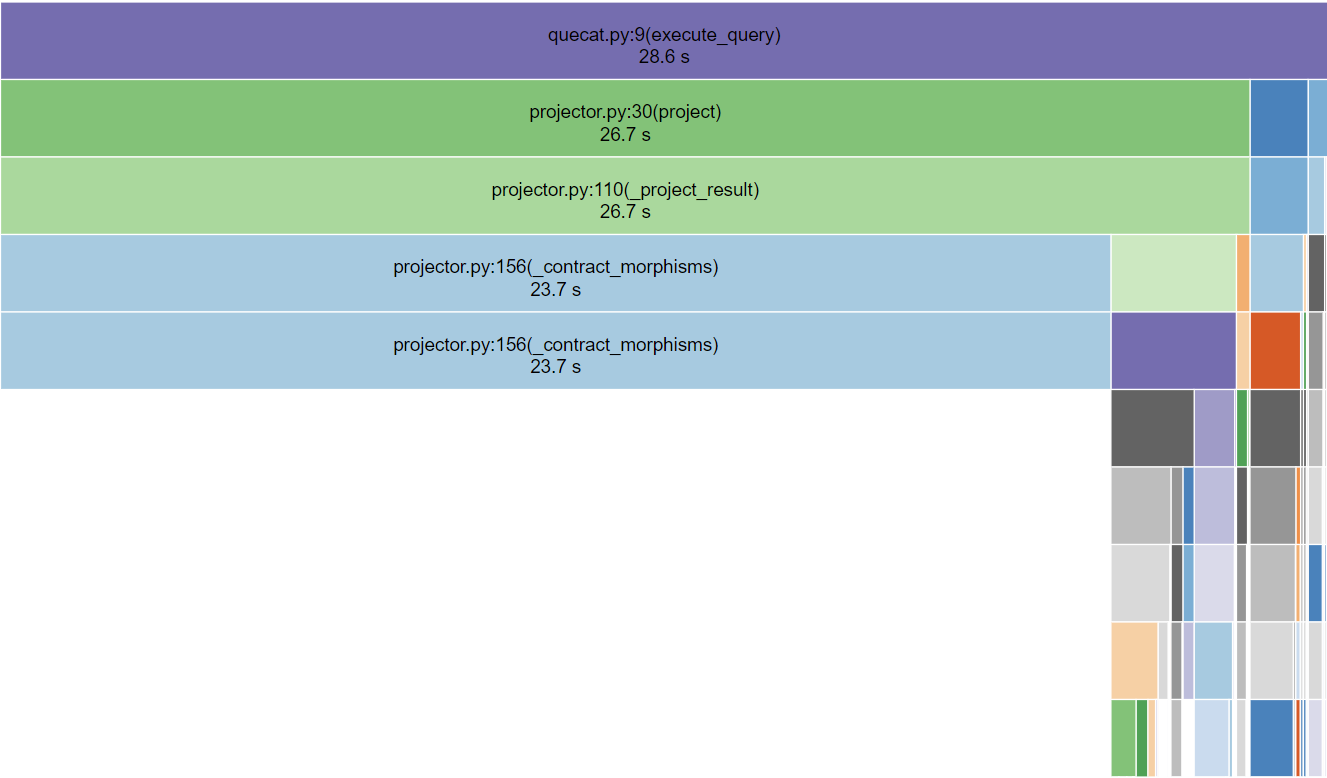
\includegraphics[width=\textwidth]{img/eval-multimodel-profile.png} 
\caption{Profiler data for the multi-model scenario.}
\label{fig:evalmultimodelprofile}
\end{figure}

Examining the profiler data shown in~\cref{fig:evalmultimodelprofile}, we can see a similar image as in~\cref{eval:subsection:mongodb}.
Again, the vast majority of the query execution time is spent on instance morphism contraction, this time over 80\%.
In this instance, the fraction of time spent on contractions is higher, because the query itself also has more contractions to perform.
While the customer ID is not being retrieved this time, all other customer properties are, leading to additional contractions needing to be done.
This, along with the combined volume of data from both databases, explains the increase in query execution time.
Again, as discussed in~\cref{eval:subsection:mongodb}, perhaps there exist more optimized ways of doing the instance morphism contractions, which would improve the overall query performance dramatically.

In addition, we can see that the merging process between the two models does not take a significant amount of time, at least compared to the effort required to perform morphism contractions.
This makes sense, as the merging process does not need to process that much data if the joining object has a simple enough identifier, which is used for the join.
Therefore future efforts in improving the querying performance should not focus on the merging algorithm, but rather on the contraction process (and the projection in general).
In other words, for queries whose projection is trivial, performance improvements are likely to be most effective in the network communication between MM-evocat and MM-quecat, whereas for queries with non-trivial projection, improvements to the morphism contraction will yield the most benefit.
